\section{Results}

\subsection{Histograms}

\begin{figure}
    \centering
    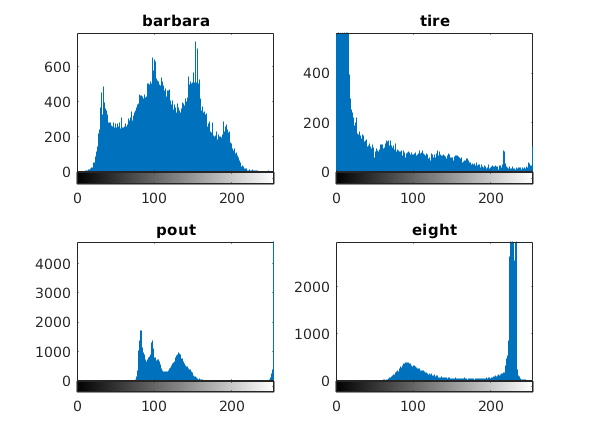
\includegraphics{histogram_compare.png}
    \caption{Histograms of Several Images}
\end{figure}

Barbara has a concentration of intensities in the middle, however has very few
at the minimum and maximum values. Tire spans the entire range of intensities,
but has a massive concentration at very dark levels. Pout has very concentrated
values around middle intensity levels, this will result in very low contrast.
Finally, eight has some values in the mid-range, but has a very large
concentration of intensity at high levels. Overall I expect tire to be the
darkest image and eight to be the brightest.

\subsection{Histogram Equalization}

\subsection{Histogram Matching}
